\part{Recurrence Relations}
\section{Handout 06: Linear Non-Homogeneous Recurrence Relations}

\subsection{Overview}

This handout completes Part~II on recurrence relations. We now study \emph{linear non-homogeneous recurrence relations with constant coefficients}. The main point is that such a recurrence is solved in two steps:
\begin{enumerate}[leftmargin=*]
    \item solve the associated homogeneous recurrence;
    \item find one particular solution of the non-homogeneous recurrence.
\end{enumerate}

The general solution is then obtained by adding these two pieces.

The main topics are:
\begin{itemize}[leftmargin=*]
    \item definition of a linear non-homogeneous recurrence relation;
    \item associated homogeneous recurrence;
    \item the structure theorem
    \[
    a_n=a_n^{(p)}+b_n;
    \]
    \item method of undetermined coefficients for polynomial forcing terms;
    \item method of undetermined coefficients for exponential forcing terms;
    \item how to modify the trial form when resonance occurs.
\end{itemize}

\begin{examtip}[title={Main workflow for Handout 06}]
To solve
\[
a_n=c_1a_{n-1}+c_2a_{n-2}+\cdots+c_ka_{n-k}+F(n),
\]
use the following order:
\begin{enumerate}[leftmargin=*]
    \item solve the associated homogeneous recurrence;
    \item guess a suitable particular solution \(a_n^{(p)}\);
    \item substitute to determine the unknown coefficients;
    \item add the homogeneous part;
    \item impose the initial conditions.
\end{enumerate}
\end{examtip}

%==================================================
\subsection{Linear Non-Homogeneous Recurrence Relations}
%==================================================

\begin{definition}{Linear non-homogeneous recurrence relation}{nonhomogeneous-def}
A \emph{linear non-homogeneous recurrence relation of degree \(k\) with constant coefficients} is a recurrence of the form
\[
a_n=c_1a_{n-1}+c_2a_{n-2}+\cdots+c_ka_{n-k}+F(n),
\]
where \(c_1,\dots,c_k\) are real constants, \(c_k\neq 0\), and \(F(n)\neq 0\) depends only on \(n\).
\end{definition}

\begin{definition}{Associated homogeneous recurrence}{associated-homogeneous}
The \emph{associated homogeneous recurrence relation} of
\[
a_n=c_1a_{n-1}+c_2a_{n-2}+\cdots+c_ka_{n-k}+F(n)
\]
is obtained by removing the forcing term \(F(n)\):
\[
b_n=c_1b_{n-1}+c_2b_{n-2}+\cdots+c_kb_{n-k}.
\]
\end{definition}

\begin{examplebox}[title={Examples}]
\[
f_n=f_{n-1}+f_{n-2}+3
\]
has associated homogeneous recurrence
\[
b_n=b_{n-1}+b_{n-2}.
\]

\[
a_n=3a_{n-1}+5a_{n-2}+n^2
\]
has associated homogeneous recurrence
\[
b_n=3b_{n-1}+5b_{n-2}.
\]

\[
a_n=2a_{n-1}-5a_{n-3}-2^n+n^2-5
\]
has associated homogeneous recurrence
\[
b_n=2b_{n-1}-5b_{n-3}.
\]
\end{examplebox}

\begin{commonmistake}[title={Adding two non-homogeneous solutions}]
If \((a_n)\) and \((d_n)\) are both solutions of the same non-homogeneous recurrence
\[
x_n=c_1x_{n-1}+\cdots+c_kx_{n-k}+F(n),
\]
then \((a_n+d_n)\) is \emph{not} generally a solution, because the forcing term becomes
\[
2F(n).
\]
This differs from the homogeneous case.
\end{commonmistake}

\begin{extension}[title={What survives from the homogeneous theory}]
The homogeneous solutions still form a vector space. The non-homogeneous solutions do not. Instead, the set of non-homogeneous solutions is a translate of the homogeneous solution space by any one particular solution.
\end{extension}

%==================================================
\subsection{Structure Theorem}
%==================================================

\begin{theorem}{General form of all solutions}{structure-theorem}
Consider
\[
a_n=c_1a_{n-1}+c_2a_{n-2}+\cdots+c_ka_{n-k}+F(n).
\]
If \(\bigl(a_n^{(p)}\bigr)\) is one particular solution of this recurrence, then every solution is of the form
\[
a_n=a_n^{(p)}+b_n,
\]
where \((b_n)\) is a solution of the associated homogeneous recurrence
\[
b_n=c_1b_{n-1}+c_2b_{n-2}+\cdots+c_kb_{n-k}.
\]
\end{theorem}

\begin{proof}
Let \((d_n)\) be any solution of the non-homogeneous recurrence. Then
\[
d_n=c_1d_{n-1}+c_2d_{n-2}+\cdots+c_kd_{n-k}+F(n),
\]
while the particular solution satisfies
\[
a_n^{(p)}=c_1a_{n-1}^{(p)}+c_2a_{n-2}^{(p)}+\cdots+c_ka_{n-k}^{(p)}+F(n).
\]
Subtracting gives
\[
d_n-a_n^{(p)}
=
c_1(d_{n-1}-a_{n-1}^{(p)})
+\cdots+
c_k(d_{n-k}-a_{n-k}^{(p)}).
\]
Hence the sequence
\[
b_n=d_n-a_n^{(p)}
\]
satisfies the associated homogeneous recurrence. Therefore
\[
d_n=a_n^{(p)}+b_n.
\]
Conversely, if \(b_n\) satisfies the associated homogeneous recurrence, then \(a_n^{(p)}+b_n\) satisfies the original non-homogeneous recurrence by direct substitution.
\end{proof}

\begin{keyformula}[title={General solution of a linear non-homogeneous recurrence}]
\[
\boxed{
\text{general solution}
=
\text{particular solution}
+
\text{general homogeneous solution}.
}
\]
\end{keyformula}

% Schematic decomposition of a non-homogeneous solution.
\begin{center}
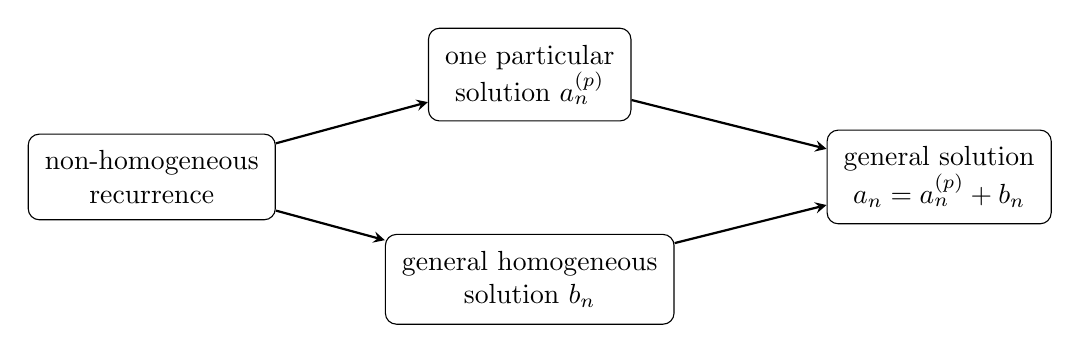
\begin{tikzpicture}[>=stealth]
    \node[draw,rounded corners,align=center,inner sep=6pt] (A) at (0,0) {non-homogeneous\\recurrence};
    \node[draw,rounded corners,align=center,inner sep=6pt] (B) at (4.8,1.3) {one particular\\solution \(a_n^{(p)}\)};
    \node[draw,rounded corners,align=center,inner sep=6pt] (C) at (4.8,-1.3) {general homogeneous\\solution \(b_n\)};
    \node[draw,rounded corners,align=center,inner sep=6pt] (D) at (10.0,0) {general solution\\\(a_n=a_n^{(p)}+b_n\)};
    \draw[->,thick] (A) -- (B);
    \draw[->,thick] (A) -- (C);
    \draw[->,thick] (B) -- (D);
    \draw[->,thick] (C) -- (D);
\end{tikzpicture}
\end{center}

\begin{examtip}[title={Why this theorem matters}]
One never needs to find \emph{all} non-homogeneous solutions directly. It is enough to find:
\begin{itemize}[leftmargin=*]
    \item one particular solution;
    \item the full homogeneous solution.
\end{itemize}
\end{examtip}

%==================================================
\subsection{A First Worked Example: Polynomial Forcing}
%==================================================

\begin{examplebox}[title={Example 10 from the handout}]
Find the solution of
\[
a_n=3a_{n-1}+2n,
\qquad a_1=3.
\]

\textbf{Step 1: Solve the associated homogeneous recurrence.}
The associated homogeneous recurrence is
\[
b_n=3b_{n-1},
\]
whose general solution is
\[
b_n=h\cdot 3^n,
\]
where \(h\) is a constant.

\textbf{Step 2: Find a particular solution.}
Here the forcing term
\[
F(n)=2n
\]
is a polynomial of degree \(1\). Since \(1\) is not a root of the homogeneous characteristic equation
\[
r-3=0,
\]
try a linear particular solution
\[
a_n^{(p)}=cn+d.
\]
Substitute:
\[
cn+d=3(c(n-1)+d)+2n.
\]
Expand:
\[
cn+d=3cn-3c+3d+2n.
\]
Move everything to one side:
\[
(2+2c)n+(2d-3c)=0.
\]
Hence
\[
2+2c=0,\qquad 2d-3c=0.
\]
So
\[
c=-1,\qquad d=-\frac32.
\]
Thus
\[
a_n^{(p)}=-n-\frac32.
\]

\textbf{Step 3: Form the general solution.}
By the structure theorem,
\[
a_n=a_n^{(p)}+b_n
=
-n-\frac32+h\cdot 3^n.
\]

\textbf{Step 4: Use the initial condition.}
Since \(a_1=3\),
\[
3=-1-\frac32+3h,
\]
so
\[
3h=\frac{11}{2}
\qquad\Longrightarrow\qquad
h=\frac{11}{6}.
\]
Therefore
\[
\boxed{
a_n=-n-\frac32+\frac{11}{6}\,3^n.
}
\]
\end{examplebox}

\begin{examplebox}[title={Second polynomial example from the handout}]
Find the solution of
\[
a_n=-2a_{n-1}+n+1,
\qquad a_0=2.
\]

The associated homogeneous recurrence is
\[
b_n=-2b_{n-1},
\]
so
\[
b_n=h(-2)^n.
\]

Since \(F(n)=n+1\) is a polynomial of degree \(1\), and \(1\) is not a root of the characteristic equation
\[
r+2=0,
\]
try
\[
a_n^{(p)}=cn+d.
\]
Substitute:
\[
cn+d=-2(c(n-1)+d)+n+1.
\]
Expand:
\[
cn+d=-2cn+2c-2d+n+1.
\]
Rearranging gives
\[
(1-3c)n+(1+2c-3d)=0.
\]
Hence
\[
1-3c=0,\qquad 1+2c-3d=0.
\]
So
\[
c=\frac13,\qquad d=\frac59.
\]
Thus
\[
a_n^{(p)}=\frac{n}{3}+\frac59.
\]
Hence the general solution is
\[
a_n=\frac{n}{3}+\frac59+h(-2)^n.
\]
Using \(a_0=2\),
\[
2=\frac59+h,
\]
so
\[
h=\frac{13}{9}.
\]
Therefore
\[
\boxed{
a_n=\frac{n}{3}+\frac59+\frac{13}{9}(-2)^n.
}
\]
\end{examplebox}

%==================================================
\subsection{Polynomial Forcing Terms}
%==================================================

The handout gives a standard guessing rule when \(F(n)\) is a polynomial.

\begin{theorem}{Trial form for polynomial forcing}{poly-trial}
Suppose
\[
a_n=c_1a_{n-1}+c_2a_{n-2}+\cdots+c_ka_{n-k}+F(n),
\]
where
\[
F(n)=b_tn^t+b_{t-1}n^{t-1}+\cdots+b_1n+b_0
\]
is a polynomial of degree \(t\).

\begin{enumerate}[leftmargin=*]
    \item If \(1\) is \emph{not} a root of the characteristic equation of the associated homogeneous recurrence, try
    \[
    a_n^{(p)}=p_tn^t+p_{t-1}n^{t-1}+\cdots+p_1n+p_0.
    \]
    \item If \(1\) \emph{is} a root of the characteristic equation, try
    \[
    a_n^{(p)}=n\bigl(p_tn^t+p_{t-1}n^{t-1}+\cdots+p_1n+p_0\bigr).
    \]
\end{enumerate}
\end{theorem}

\begin{keyformula}[title={Polynomial forcing rule}]
If \(F(n)\) is polynomial of degree \(t\), then:
\[
\text{try degree }t
\quad\text{or}\quad
n\times\text{degree }t
\]
according to whether \(1\) is not a root or is a root of the characteristic equation.
\end{keyformula}

\begin{examplebox}[title={Handout question: what should we try?}]
Suppose
\[
a_n=a_{n-1}+n.
\]
What trial form should be used?

The associated homogeneous recurrence is
\[
b_n=b_{n-1},
\]
whose characteristic equation is
\[
r-1=0.
\]
Thus \(1\) is a root. Since the forcing term \(n\) is a polynomial of degree \(1\), the correct trial is
\[
a_n^{(p)}=n(cn+d)=cn^2+dn.
\]
\end{examplebox}

\begin{commonmistake}[title={Forgetting the extra factor \(n\)}]
If \(1\) is a root of the characteristic equation, then a plain polynomial trial overlaps with the homogeneous solution and fails. One must multiply by \(n\).

\end{commonmistake}

\begin{extension}[title={Resonance viewpoint for polynomial forcing}]
The special role of \(1\) comes from the fact that polynomial sequences are built from powers of \(n\), while the homogeneous solution corresponding to root \(1\) contains constant-type behaviour. Multiplying by \(n\) shifts the trial form out of the homogeneous solution space.
\end{extension}

%==================================================
\subsection{Exponential Forcing Terms}
%==================================================

We now consider forcing terms of the form
\[
F(n)=s^n.
\]

\begin{theorem}{Trial form for exponential forcing}{exp-trial}
Suppose
\[
a_n=c_1a_{n-1}+c_2a_{n-2}+\cdots+c_ka_{n-k}+s^n.
\]

\begin{enumerate}[leftmargin=*]
    \item If \(s\) is \emph{not} a root of the characteristic equation of the associated homogeneous recurrence, try
    \[
    a_n^{(p)}=c\,s^n.
    \]
    \item If \(s\) \emph{is} a root of the characteristic equation, try
    \[
    a_n^{(p)}=c\,n\,s^n.
    \]
\end{enumerate}
\end{theorem}

\begin{keyformula}[title={Exponential forcing rule}]
For \(F(n)=s^n\), try
\[
c\,s^n
\quad\text{or}\quad
c\,n\,s^n
\]
according to whether \(s\) is not a root or is a root of the homogeneous characteristic equation.
\end{keyformula}
\begin{examplebox}[title={Example 11 from the handout}]
Find all solutions of
\[
a_n=5a_{n-1}-6a_{n-2}+7^n.
\]

\textbf{Step 1: Solve the associated homogeneous recurrence.}
The associated homogeneous recurrence is
\[
b_n=5b_{n-1}-6b_{n-2}.
\]
Its characteristic equation is
\[
r^2-5r+6=0=(r-2)(r-3),
\]
so
\[
b_n=h_1\,2^n+h_2\,3^n.
\]

\textbf{Step 2: Find a particular solution.}
Since the forcing term is \(7^n\), and \(7\) is not a root of the characteristic equation, try
\[
a_n^{(p)}=c\,7^n.
\]
Substitute:
\[
c7^n=5c7^{n-1}-6c7^{n-2}+7^n.
\]
Multiply through by \(7^{-(n-2)}\):
\[
49c=35c-6c+49.
\]
Hence
\[
20c=49
\qquad\Longrightarrow\qquad
c=\frac{49}{20}.
\]
Thus
\[
a_n^{(p)}=\frac{49}{20}7^n.
\]

\textbf{Step 3: Combine.}
Therefore all solutions are
\[
\boxed{
a_n=\frac{49}{20}7^n+h_1\,2^n+h_2\,3^n.
}
\]
\end{examplebox}

\begin{examplebox}[title={Handout question: what should we try?}]
Suppose
\[
a_n=5a_{n-1}+5^n.
\]
What should be tried for a particular solution?

The associated homogeneous recurrence is
\[
b_n=5b_{n-1},
\]
whose characteristic equation is
\[
r-5=0.
\]
Thus \(5\) is a root. Therefore the correct trial is
\[
a_n^{(p)}=c\,n\,5^n.
\]
\end{examplebox}

\begin{commonmistake}[title={Using \(c\,s^n\) when \(s\) is already a homogeneous root}]
If \(s\) is a root of the characteristic equation, then \(s^n\) is already part of the homogeneous solution. A trial of the form \(c\,s^n\) cannot produce a genuinely new particular solution. Multiply by \(n\).
\end{commonmistake}

%==================================================
\subsection{How Initial Conditions Enter}
%==================================================

After a particular solution and the homogeneous solution have been combined, one obtains a general expression with arbitrary constants. These are determined exactly as in the homogeneous case by substituting the given initial conditions.

\begin{examplebox}[title={Tutorial 6, Question 4(a)}]
Find all solutions of
\[
a_n=2a_{n-1}+2n^2
\qquad (n\ge 2),
\]
and then determine the solution with \(a_1=4\).

The associated homogeneous recurrence is
\[
b_n=2b_{n-1},
\]
so
\[
b_n=h\,2^n.
\]

Since \(F(n)=2n^2\) is a polynomial of degree \(2\), and \(1\) is not a root of \(r-2=0\), try
\[
a_n^{(p)}=cn^2+dn+e.
\]
Substituting into
\[
a_n=2a_{n-1}+2n^2
\]
gives
\[
c=-2,\qquad d=-8,\qquad e=-12.
\]
Hence
\[
a_n^{(p)}=-2n^2-8n-12.
\]
So all solutions are
\[
a_n=h\,2^n-2n^2-8n-12.
\]
Using \(a_1=4\),
\[
4=2h-22,
\]
hence
\[
h=13.
\]
Therefore
\[
\boxed{
a_n=13\cdot 2^n-2n^2-8n-12.
}
\]
\end{examplebox}

\begin{examplebox}[title={Tutorial 6, Question 5(b)}]
Find all solutions of
\[
a_n=4a_{n-1}-3a_{n-2}+3^n.
\]

The associated homogeneous recurrence is
\[
b_n=4b_{n-1}-3b_{n-2},
\]
whose characteristic equation is
\[
r^2-4r+3=0=(r-1)(r-3).
\]
So
\[
b_n=h_1+h_2\,3^n.
\]

Since the forcing term is \(3^n\), and \(3\) is a root of the characteristic equation, try
\[
a_n^{(p)}=c\,n\,3^n.
\]
Substitute:
\[
cn3^n=4c(n-1)3^{n-1}-3c(n-2)3^{n-2}+3^n.
\]
Dividing by \(3^{n-2}\) gives
\[
9cn=12c(n-1)-3c(n-2)+9.
\]
Simplifying,
\[
9cn=9cn-6c+9,
\]
so
\[
6c=9
\qquad\Longrightarrow\qquad
c=\frac32.
\]
Therefore
\[
a_n^{(p)}=\frac32\,n\,3^n.
\]
Hence all solutions are
\[
\boxed{
a_n=h_1+h_2\,3^n+\frac32\,n\,3^n.
}
\]
\end{examplebox}

%==================================================
\subsection{Special Techniques}
%==================================================

\subsubsection*{1. Separate the problem into homogeneous part + particular part}
Always identify the associated homogeneous recurrence first. The final solution is built by adding a particular solution.

\subsubsection*{2. Diagnose the forcing term before guessing}
Check whether \(F(n)\) is polynomial, exponential, or a sum of simpler terms. The trial form should reflect the shape of the forcing term.

\subsubsection*{3. Test for resonance}
If the obvious trial overlaps with the homogeneous solution, multiply by \(n\). In this handout:
\begin{itemize}[leftmargin=*]
\item polynomial forcing is sensitive to whether \(1\) is a root;
\item exponential forcing \(s^n\) is sensitive to whether \(s\) is a root.
\end{itemize}

\subsubsection*{4. Use linearity of forcing when appropriate}
If the forcing term splits as
\[
F(n)=F_1(n)+F_2(n),
\]
and one can find particular solutions for each component separately, then their sum is a particular solution for the full recurrence.

\subsubsection*{5. Expand only as much as needed}
When comparing coefficients, collect powers of \(n\) carefully and equate coefficients systematically.

\subsubsection*{6. Keep the constants for the very end}
Do not impose initial conditions until after the full general solution
\[
a_n=a_n^{(p)}+b_n
\]
has been formed.

\begin{extension}[title={Why the method works so efficiently}]
The method of undetermined coefficients succeeds because the recurrence operator sends polynomial and exponential trial families into the same kind of families. This makes the unknown coefficients solvable by finite algebra rather than by guesswork.
\end{extension}

%==================================================
\subsection{Summary Table}
%==================================================

\begin{center}
\small
\begin{tabular}{@{}p{0.30\textwidth}p{0.28\textwidth}p{0.29\textwidth}@{}}
\toprule
\textbf{Forcing term \(F(n)\)} & \textbf{Condition} & \textbf{Trial for \(a_n^{(p)}\)} \\
\midrule
Polynomial of degree \(t\) & \(1\) not a root & degree-\(t\) polynomial \\
Polynomial of degree \(t\) & \(1\) is a root & \(n\times\) degree-\(t\) polynomial \\
Exponential \(s^n\) & \(s\) not a root & \(c\,s^n\) \\
Exponential \(s^n\) & \(s\) is a root & \(c\,n\,s^n\) \\
General case & one particular solution known & \(a_n=a_n^{(p)}+b_n\) \\
\bottomrule
\end{tabular}
\end{center}

\begin{examtip}[title={Final checklist for Handout 06}]
Before finalizing a solution, check:
\begin{enumerate}[leftmargin=*]
    \item Have I written the associated homogeneous recurrence correctly?
    \item Have I chosen a trial form that matches the forcing term?
    \item Have I checked whether an extra factor of \(n\) is needed?
    \item Have I found one particular solution correctly?
    \item Have I added the general homogeneous solution?
    \item Have I used the initial conditions only at the final stage?
\end{enumerate}
\end{examtip}

\begin{commonmistake}[title={Solving only the homogeneous part}]
A homogeneous solution alone is not a solution to the non-homogeneous recurrence unless the forcing term vanishes. One must always include a particular solution.
\end{commonmistake}